\documentclass[tikz,border=6pt]{standalone}
\usepackage[T1]{fontenc}
\usepackage[utf8]{inputenc}
\usepackage{import}
\subimport{layers/}{init.tex}
\usetikzlibrary{arrows.meta,positioning}
\definecolor{ink}{HTML}{242629}
\definecolor{muted}{HTML}{59616a}
\definecolor{panel}{HTML}{f6f6f3}
\definecolor{blue}{HTML}{dfeaf5}
\definecolor{peach}{HTML}{f7cdae}
\definecolor{green}{HTML}{a9ce91}
\definecolor{yellow}{HTML}{ffe49b}
\definecolor{purple}{HTML}{d5c5e8}
\definecolor{white}{HTML}{ffffff}
\definecolor{heat}{HTML}{e89a50}
\definecolor{offset}{HTML}{a6bdd8}
\definecolor{size}{HTML}{ddc66e}
\definecolor{yaw}{HTML}{a8c983}
\definecolor{iou}{HTML}{b6a1cd}
\begin{document}
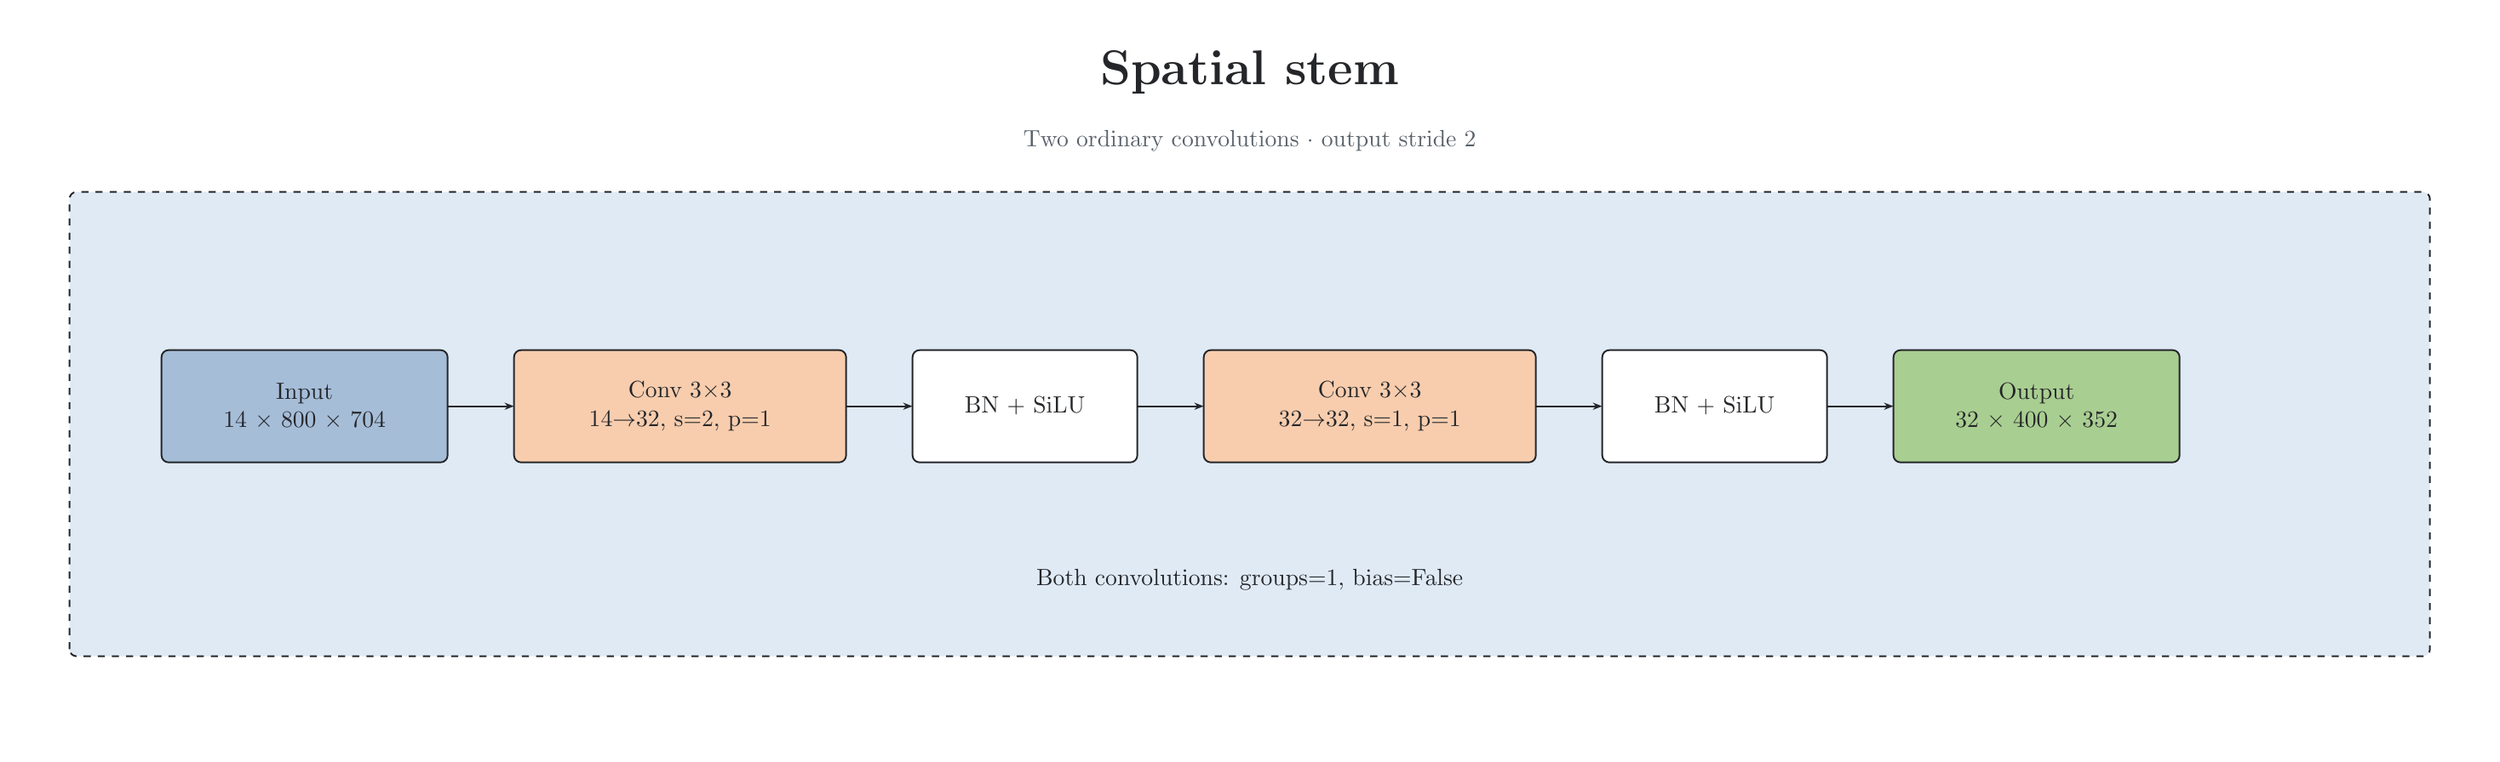
\begin{tikzpicture}[x=1.524cm,y=1.524cm,z={(0.9906cm,0.73152cm)}]
\path[use as bounding box] (0,0) rectangle (24,7);
\node[anchor=center,align=center,text=ink,font=\fontsize{20}{24.0}\selectfont \bfseries ] at (12.0,6.52) {Spatial stem};
\node[anchor=center,align=center,text=muted,font=\fontsize{10}{12.0}\selectfont ] at (12.0,5.85) {Two ordinary convolutions $\cdot$ output stride 2};
\draw[draw=ink,fill=blue,rounded corners=3pt,line width=.7pt,dashed] (0.4499999999999993,0.8000000000000003) rectangle (23.55,5.35);
\node[anchor=west,align=left,text=ink,font=\fontsize{15}{18.0}\selectfont \bfseries ] at (0.8,4.85) {};
\draw[draw=ink,fill=offset,rounded corners=3pt,line width=.7pt] (1.35,2.7) rectangle (4.15,3.8);
\node[anchor=center,align=center,text=ink,font=\fontsize{10}{12.0}\selectfont ] at (2.75,3.25) {Input\\14 $\times$ 800 $\times$ 704};
\draw[-{Stealth[length=4pt]},draw=ink,line width=.7pt] (4.15,3.25) -- (4.800000000000001,3.25);
\draw[draw=ink,fill=peach,rounded corners=3pt,line width=.7pt] (4.800000000000001,2.7) rectangle (8.05,3.8);
\node[anchor=center,align=center,text=ink,font=\fontsize{10}{12.0}\selectfont ] at (6.425000000000001,3.25) {Conv 3$\times$3\\14$\rightarrow$32, s=2, p=1};
\draw[-{Stealth[length=4pt]},draw=ink,line width=.7pt] (8.05,3.25) -- (8.700000000000001,3.25);
\draw[draw=ink,fill=white,rounded corners=3pt,line width=.7pt] (8.700000000000001,2.7) rectangle (10.9,3.8);
\node[anchor=center,align=center,text=ink,font=\fontsize{10}{12.0}\selectfont ] at (9.8,3.25) {BN + SiLU};
\draw[-{Stealth[length=4pt]},draw=ink,line width=.7pt] (10.900000000000002,3.25) -- (11.550000000000002,3.25);
\draw[draw=ink,fill=peach,rounded corners=3pt,line width=.7pt] (11.550000000000002,2.7) rectangle (14.800000000000002,3.8);
\node[anchor=center,align=center,text=ink,font=\fontsize{10}{12.0}\selectfont ] at (13.175000000000002,3.25) {Conv 3$\times$3\\32$\rightarrow$32, s=1, p=1};
\draw[-{Stealth[length=4pt]},draw=ink,line width=.7pt] (14.800000000000002,3.25) -- (15.450000000000003,3.25);
\draw[draw=ink,fill=white,rounded corners=3pt,line width=.7pt] (15.450000000000005,2.7) rectangle (17.650000000000006,3.8);
\node[anchor=center,align=center,text=ink,font=\fontsize{10}{12.0}\selectfont ] at (16.550000000000004,3.25) {BN + SiLU};
\draw[-{Stealth[length=4pt]},draw=ink,line width=.7pt] (17.650000000000002,3.25) -- (18.3,3.25);
\draw[draw=ink,fill=green,rounded corners=3pt,line width=.7pt] (18.3,2.7) rectangle (21.099999999999998,3.8);
\node[anchor=center,align=center,text=ink,font=\fontsize{10}{12.0}\selectfont ] at (19.7,3.25) {Output\\32 $\times$ 400 $\times$ 352};
\node[anchor=center,align=center,text=ink,font=\fontsize{10}{12.0}\selectfont ] at (12,1.55) {Both convolutions: groups=1, bias=False};
\end{tikzpicture}
\end{document}
